\documentclass[11pt]{beamer}
\usetheme{Dresden}
%\usecolortheme{beaver}
\usepackage[utf8]{inputenc}
\usepackage{amsmath}
\usepackage{amsfonts}
\usepackage{amssymb}
\usepackage{graphicx}
\usepackage{listings}
\usepackage{verbatim}
\author{Zheng Zheng}
\title{Topic 12 - Data Structures}
%\setbeamercovered{transparent} 
%\setbeamertemplate{navigation symbols}{} 
%\logo{} 
\institute{McMaster University}
\date{Winter 2023} 
\subject{COMPSCI 1XC3 - Computer Science Practice and Experience:
Development Basics} 
\stepcounter{section}

\definecolor{mGreen}{rgb}{0,0.6,0}
\definecolor{mGray}{rgb}{0.5,0.5,0.5}
\definecolor{mPurple}{rgb}{0.58,0,0.05}
\definecolor{mGreen2}{rgb}{0.05,0.65,0.05}
\definecolor{mGray2}{rgb}{0.55,0.55,0.55}
\definecolor{mPurple2}{rgb}{0.63,0.05,0.05}
\definecolor{backgroundColour}{rgb}{0.95,0.95,0.92}
\definecolor{backgroundColour2}{rgb}{0.95,0.92,0.95}

\lstdefinestyle{C}{
    backgroundcolor=\color{backgroundColour},   
    commentstyle=\color{mGreen},
    keywordstyle=\color{blue},
    numberstyle=\tiny\color{mGray},
    stringstyle=\color{mPurple},    
    basicstyle=\footnotesize,
    breakatwhitespace=false,         
    breaklines=true,                 
    captionpos=b,                    
    keepspaces=true,                 
    numbers=left,                    
    numbersep=5pt,                  
    showspaces=false,                
    showstringspaces=false,
    showtabs=false,                  
    tabsize=2,
    language=C
}

\definecolor{eggplant}{rgb}{0.52,0.11,0.3} 

\usecolortheme[named=eggplant]{structure}

\begin{document}

\begin{frame}
\center
COMPSCI 1XC3 - Computer Science Practice and Experience:
Development Basics
\titlepage
% Adapted from Chapters 10 and 12 of C: How to Program 8th ed., Deitel \& Deitel
\end{frame}

\begin{frame}
\tableofcontents
\end{frame}

\section[struct]{Structured Programming}
\begin{frame}[fragile=singleslide]{Gettting Structure in your life}
Up to this point, we have had no abstraction mechanisms in C besides functions. Consider the following scenario...
\begin{itemize}
\item Let's imagine we have a database that contains the names, email addresses, and pinball high scores of customers, stored as a CSV file:
\end{itemize}
\begin{verbatim}
"John Boring","john.boring@whatever.com",100000
"Sally Plain","sally.plain@whatever.com",200000
"Nancy Snore","nancy.snore@whatever.com",50000
"Peter Bland","peter.bland@whatever.com",150000
"Thamarias the High Elf","Elder.Cabbage@
  ancientorderofpurplewizards.com",999999999
\end{verbatim}
We could group this data by field into arrays, or, we could use \texttt{struct} to make a record data type!  
\end{frame}

\begin{frame}[fragile=singleslide]{Introducing... \texttt{struct}!}
\begin{itemize}
\item A structure groups several variables together into a single data type.
\item Structures are roughly analogous to classes in Python, if you remove the methods.
\end{itemize}
\begin{lstlisting}[style=C]
struct customer {
	char *name;
	char *email;
	int pinball;
} ; 
\end{lstlisting}
\begin{itemize}
\item This creates a new data type, \texttt{customer}, with the \textbf{fields} \texttt{name}, \texttt{email} and \texttt{pinball}.
\end{itemize}
\end{frame}

\begin{frame}[fragile=singleslide]{Working with Structs}
The fields of a structure are accessed through \textbf{dot syntax}.
\begin{lstlisting}[style=C]
	struct customer ma_bois[5];
	ma_bois[0].name = "John Boring";
	ma_bois[0].email = "john.boring@whatever.com";
	ma_bois[0].pinball = 100000;
	struct customer ma_boi = {"Sally Plain"
							,"sally.plain@whatever.com"
							,200000 };
	printf("%s, %s, %d\n"
	      , ma_bois[0].name
	      , ma_bois[0].email
	      , ma_bois[0].pinball);
\end{lstlisting}
You can also initialize a structure in a similar manner to an array (line 5 above).
\end{frame}

\begin{frame}[fragile=singleslide]{Some Quality of Life Improvements}
We can avoid having to invoke the \texttt{struct} keyword when declaring a variable using our new structures.  Simply include the following in the global namespace:
\begin{lstlisting}[style=C]
typedef struct customer Customer;
\end{lstlisting}
We can also define a default structure variable as follows:
\begin{lstlisting}[style=C]
struct customer {
	char *name;
	char *email;
	int pinball;
} cust_def = {"None", "None", 0};
\end{lstlisting}
This allows us to use \texttt{cust\_def} whenever we want to initialize or reset a record:
\begin{lstlisting}[style=C]
	Customer ma_bois[5] = {cust_def,cust_def,cust_def,cust_def,cust_def} ;
\end{lstlisting}
\end{frame}

\begin{frame}{Additional Notes on Structures}
\begin{itemize}
\item Structure members may be variables of primitive data types, or aggregate data types, such as arrays or other structures.
\item A structure may \emph{not} contain an instance of itself.
\item A structure may contain a \emph{pointer to} an object of the same type as the structure
\begin{itemize}
\item Many advanced data structures, such as trees, rely on this.
\item This is a \textbf{recursive} ir \textbf{self-referential} data structure.
\end{itemize}
\item You may declare any number of variables after a structure definition, not just the default shown on the previous slide. 
\item You may even omit the strucutre tag (in our case \texttt{customer}), and declare all of your variables in the global namespace.  
\end{itemize}
\end{frame}

\begin{frame}{Valid Operations on Structures}
Unlike classes in Python (and other object oriented languages), structures have a relatively small number of operations which may be performed on them:
\begin{itemize}
\item Assignment (\texttt{=})
\item Address of (\texttt{\&})
\item Finding Bit Width with \texttt{sizeof()}
\begin{itemize}
\item The size of a structure is (roughly) the sum of the sizes of all its fields.  
\item Sometimes, blank space may be included due to the addressing of small variables.
\end{itemize}
\end{itemize}
NOTE: These are operations on variables of the structure type, not fields of the structure.
\end{frame}

\begin{frame}{A Longer Example}
\center
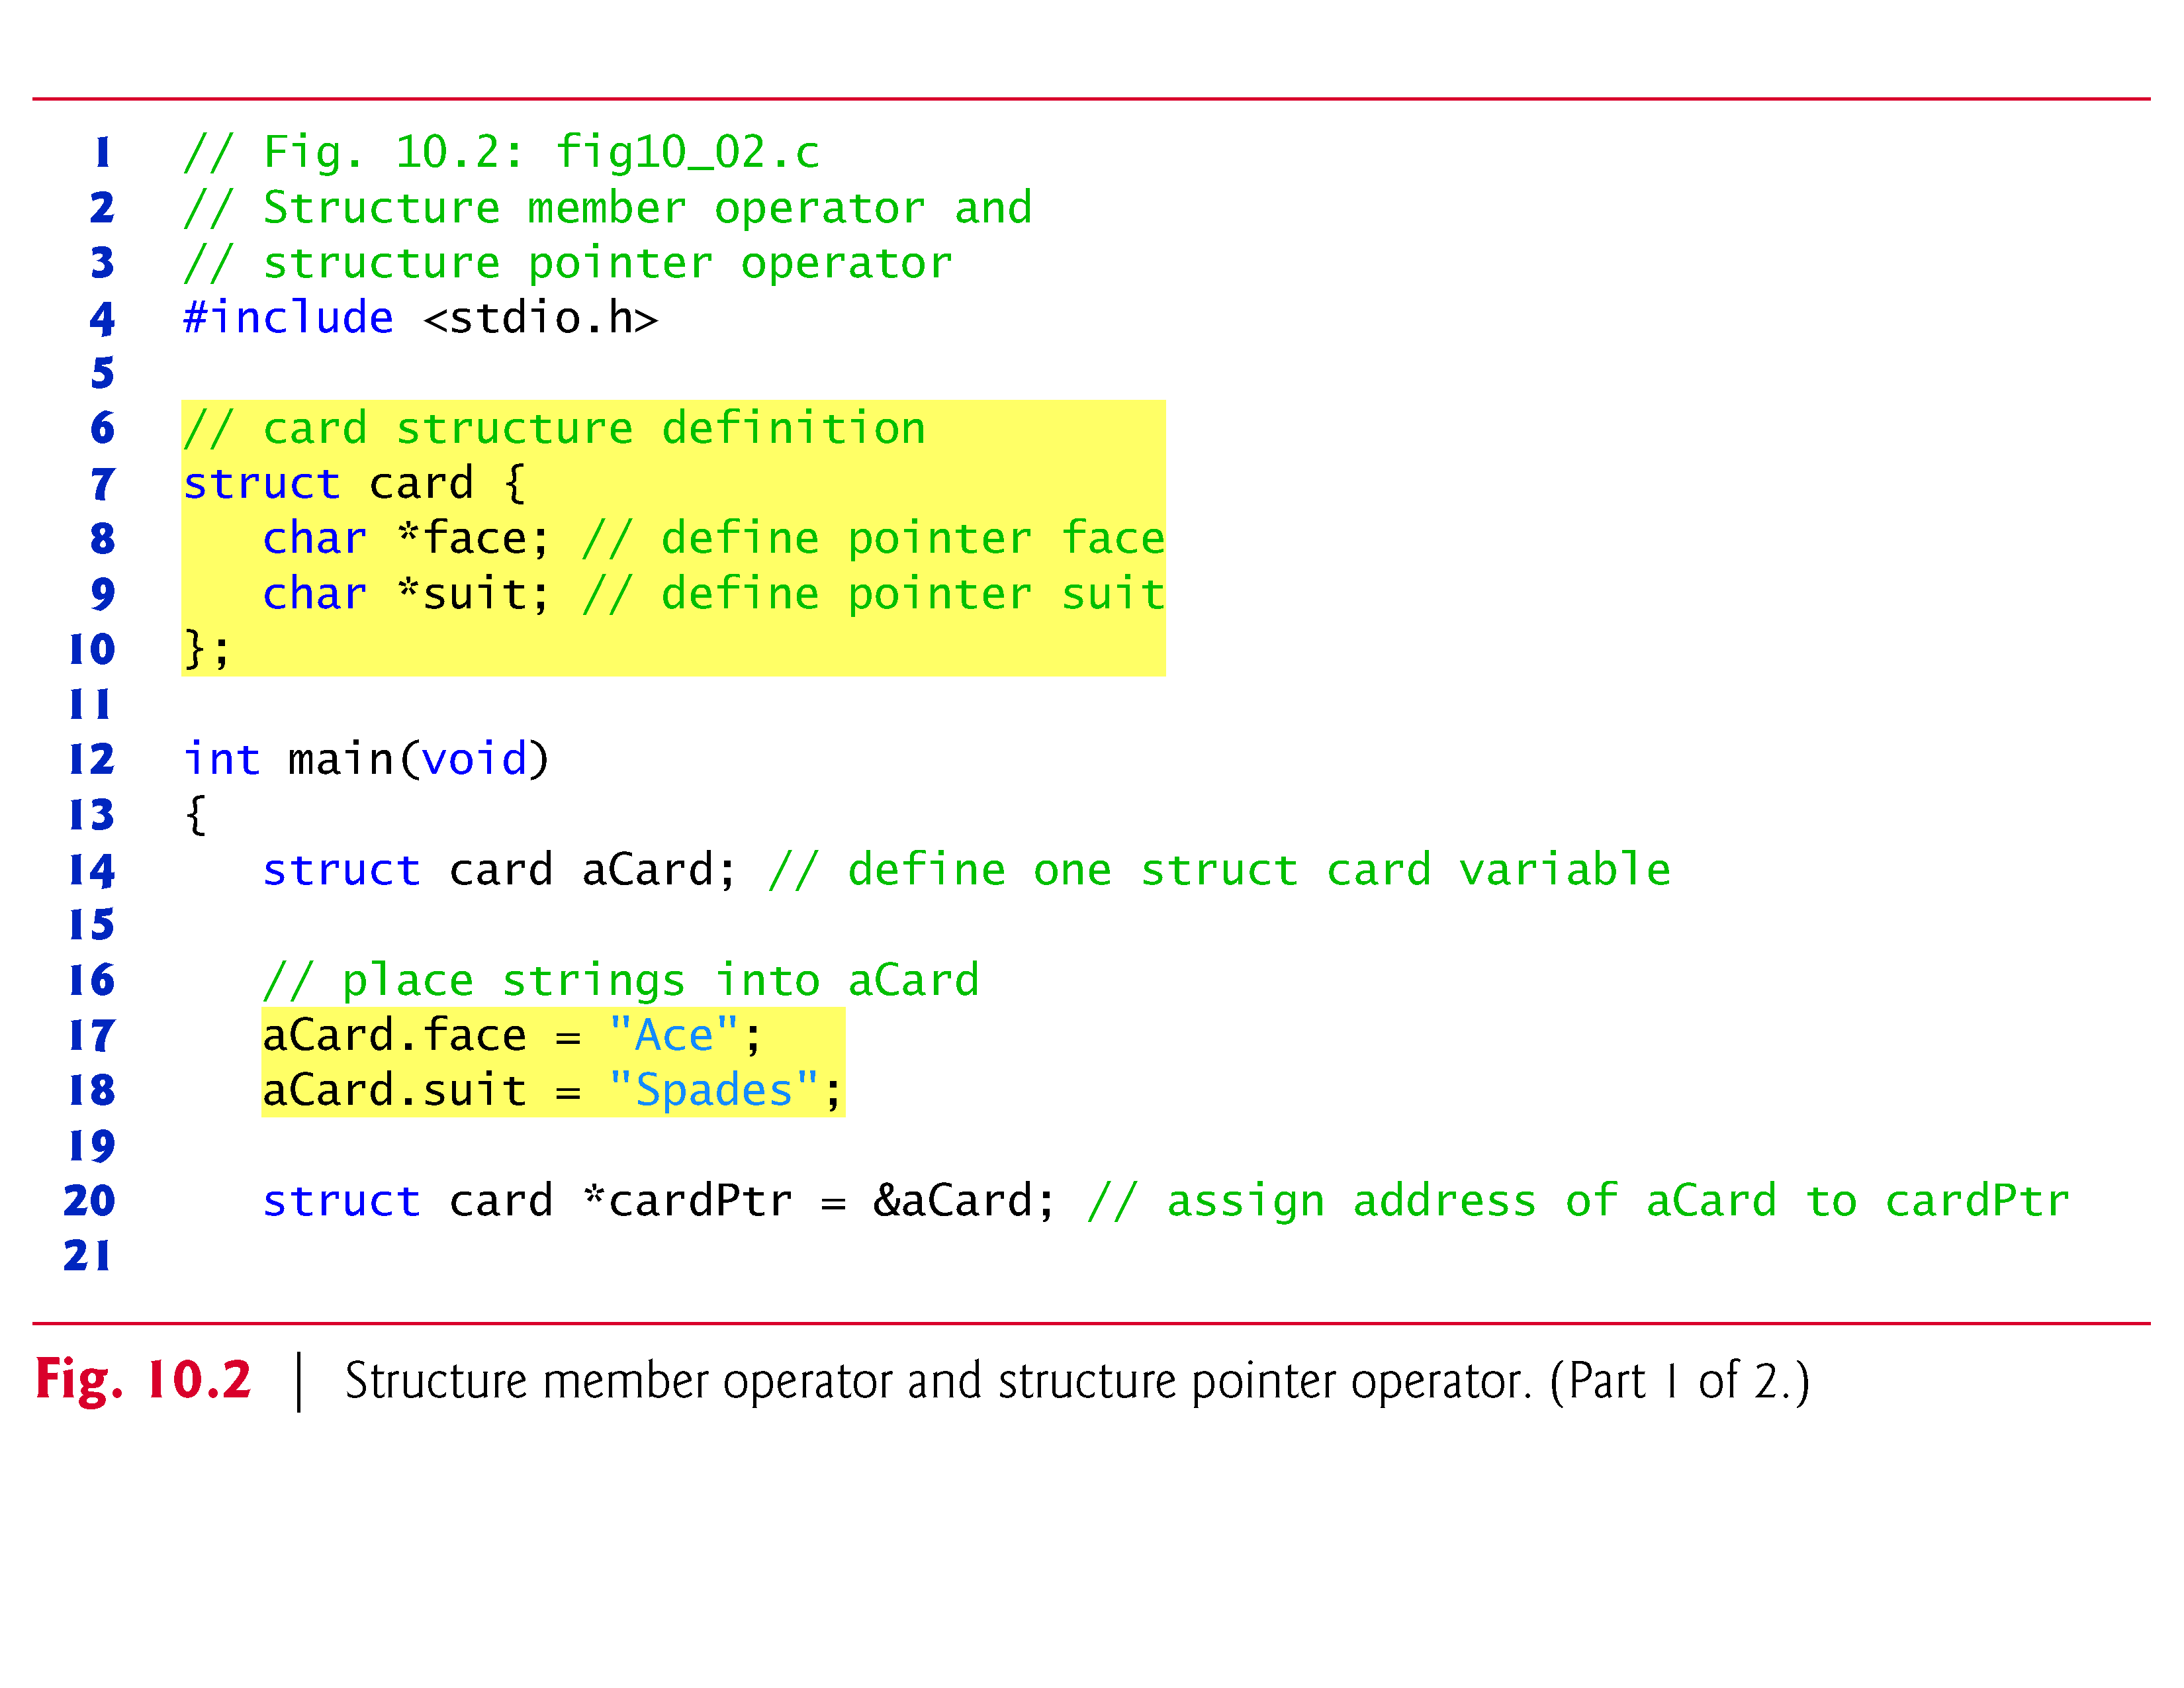
\includegraphics[scale=0.35]{struct1.png}
\end{frame}

\begin{frame}{A Longer Example (cont.)}
\center
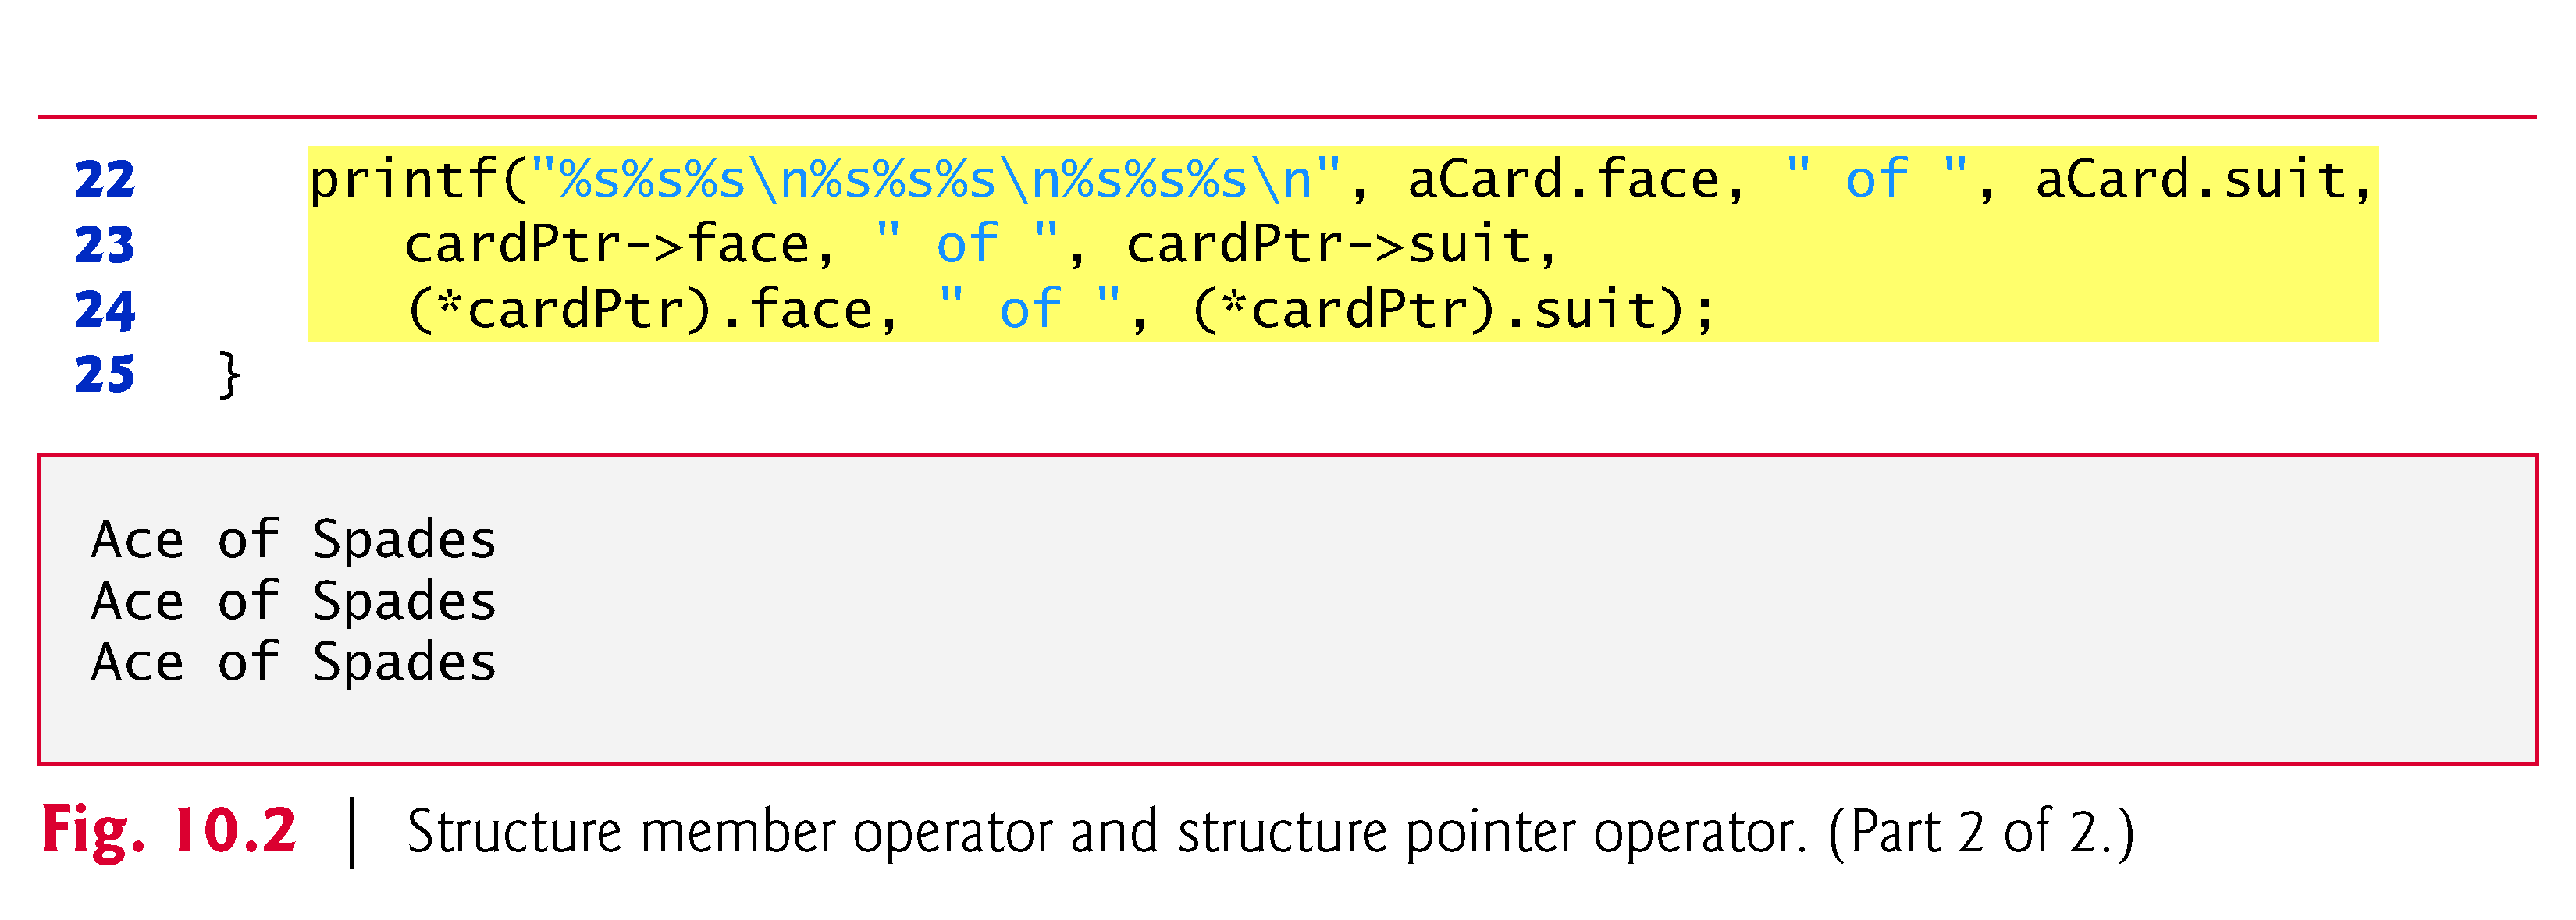
\includegraphics[scale=0.12]{struct2.png}
\end{frame}

\begin{frame}{Structures + Pointers = Love}
In the previous example, you may have noticed a pointer to a structure type.
\begin{itemize}
\item When you have a pointer to a structure, you access the fields of the structure pointed to using \texttt{-\textgreater}
\item This is syntactic sugar for pointer dereferencing and field access, combined into one operator:
\begin{itemize}
\item \texttt{x -\textgreater y} $\equiv$ \texttt{(*x).y}
\end{itemize}
\item It is almost always more efficient to pass structures \emph{by reference} rather than \emph{by value}
\item You can allocate memory to a structure pointer the same way as everything else: using \texttt{malloc()} or \texttt{calloc()}.
\begin{itemize}
\item Don't forget to \texttt{free()}!
\end{itemize}
\end{itemize}
\end{frame}

\section[Bitwise]{Bitwise Operations}
\begin{frame}{And Here's Some Bitwise Apropos of Nothing}
Bitwise operators will become very important when you start working with embedded systems, so let's review them! 
\begin{itemize}
\item \texttt{\&} - bitwise and
\item \texttt{\textbar} - bitwise or
\item \texttt{\textasciicircum} - bitwise xor
\item \texttt{\textless\textless} - bitwise left shift
\item \texttt{\textgreater\textgreater} - bitwise right shift
\item \texttt{\textasciitilde} - bitwise complement
\end{itemize}
``Bitwise'' means ``by the bit,'' where individual bits are the values under consideration, as we shall see...
\end{frame}

\begin{frame}{And}
\begin{columns}
\begin{column}{0.7\textwidth}
Bitwise AND may be thought of as the application of a logical AND gate to each of the bits in the two operands sequentially. Common C applications include bitmasking.   
\center
\begin{tabular}{| c | c | c |}
\hline
x & y & x \& y \\ \hline
1 & 1 & 1 \\ \hline
0 & 1 & 0 \\ \hline
1 & 0 & 0 \\ \hline
0 & 0 & 0 \\ \hline
\end{tabular}

\begin{tabular}{| c | c | c |}
\hline
Variable & Dec & Binary \\ \hline
\texttt{x} & 51 & \texttt{0b00110011} \\ \hline
\texttt{y} & 85 & \texttt{0b01010101} \\ \hline
\texttt{x \& y} & 17 & \texttt{0b00010001} \\ \hline
\end{tabular}

\end{column}
\begin{column}{0.3\textwidth}
\center
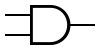
\includegraphics[scale=0.5]{andgate.png}

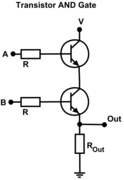
\includegraphics[scale=0.8]{TransistorANDgate.png}
\end{column}
\end{columns}
\end{frame}

\begin{frame}{Or}
\begin{columns}
\begin{column}{0.7\textwidth}
Bitwise OR is applied in the same manner, but uses a logical OR operation.  
\center
\begin{tabular}{| c | c | c |}
\hline
x & y & x \textbar y \\ \hline
1 & 1 & 1 \\ \hline
0 & 1 & 1 \\ \hline
1 & 0 & 1 \\ \hline
0 & 0 & 0 \\ \hline
\end{tabular}

\begin{tabular}{| c | c | c |}
\hline
Variable & Dec & Binary \\ \hline
\texttt{x} & 51 & \texttt{0b00110011} \\ \hline
\texttt{y} & 85 & \texttt{0b01010101} \\ \hline
\texttt{x \textbar y} & 119 & \texttt{0b01110111} \\ \hline
\end{tabular}

\end{column}
\begin{column}{0.3\textwidth}
\center
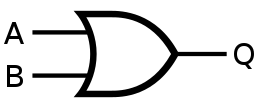
\includegraphics[scale=0.3]{orgate.png}

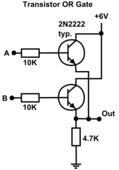
\includegraphics[scale=0.8]{transistorOrGate.png}
\end{column}
\end{columns}
\end{frame}

\begin{frame}{Xor}
\begin{columns}
\begin{column}{0.7\textwidth}
\texttt{\textasciicircum} means ``exclusive or'', outputing 1 if the inputs are dissimilar.  Common applications include bit toggling and arithmetic addition.  
\center
\begin{tabular}{| c | c | c |}
\hline
x & y & x \textasciicircum y \\ \hline
1 & 1 & 0 \\ \hline
0 & 1 & 1 \\ \hline
1 & 0 & 1 \\ \hline
0 & 0 & 0 \\ \hline
\end{tabular}

\begin{tabular}{| c | c | c |}
\hline
Variable & Dec & Binary \\ \hline
\texttt{x} & 51 & \texttt{0b00110011} \\ \hline
\texttt{y} & 85 & \texttt{0b01010101} \\ \hline
\texttt{x \textasciicircum y} & 102 & \texttt{0b01100110} \\ \hline
\end{tabular}
\end{column}
\begin{column}{0.3\textwidth}
\center
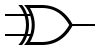
\includegraphics[scale=0.5]{xorgate.png}
\\
\vspace{2em}
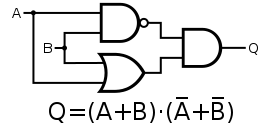
\includegraphics[scale=0.4]{xorInOtherGates.png}
\end{column}
\end{columns}
\end{frame}

\begin{frame}{Left Shift}
The left shift operation \texttt{x \textless\textless y} moves the bit values of the number x by a number of bits y to the ``left''.  
\begin{itemize}
\item We consider ``left'' to be towards larger place values, in \textbf{big endian} systems (which are most of them).
\item From a pragmatic standpoint, this is precisely the same as \emph{multiplication} by $2^{y}$  
\end{itemize}
\center 
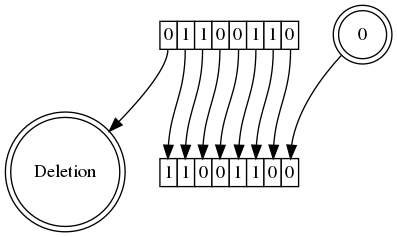
\includegraphics[scale=0.35]{ls.png}
\end{frame}

\begin{frame}{Right Shift}
The right shift operation \texttt{x \textgreater\textgreater y} moves the bit values of the number x by a number of bits y to the ``right''.  
\begin{itemize}
\item Just like the last one, but in the reverse direction.  
\item From a pragmatic standpoint, this is precisely the same as \emph{division} by $2^{y}$, with truncation.
\end{itemize}
\center 
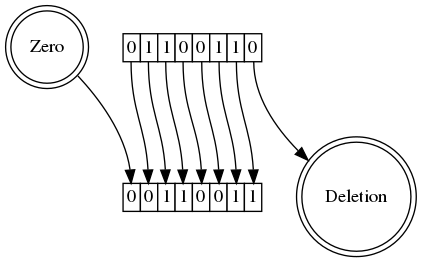
\includegraphics[scale=0.35]{rs.png}
\end{frame}

\begin{frame}{One's Complement}
The complement operator \textasciitilde simply takes each bit and flips it.  
\center
\begin{tabular}{| c | c | c |}
\hline
Variable & Dec & Binary \\ \hline
\texttt{x} & 51 & \texttt{0b00110011} \\ \hline
\texttt{\textasciitilde x} & 204 & \texttt{0b11001100} \\ \hline
\end{tabular}
\flushleft
If you're the type of nerd that likes to squeeze either speed or power efficiency out of your code, bitwise operations typically take far less circuitry (and in some cases time) than algebraic operations.  
\end{frame}

\begin{frame}[fragile=singleslide]{Some Common Operations using Bitwise}
\begin{columns}
\begin{column}{0.5\textwidth}
Subtraction using Bitwise
\begin{lstlisting}[style=C]
int subtract(int x, int y) 
{ 
	int borrow = 0;
    while (y != 0) 
    { 
        borrow = (~x) & y; 
        x = x ^ y; 
        y = borrow << 1; 
    } 
    return x; 
} 
\end{lstlisting}
\end{column}
\begin{column}{0.5\textwidth}
Addition using Bitwise
\begin{lstlisting}[style=C]
int Add(int x, int y)  
{  
	int carry = 0;
    while (y != 0)  
    {  
        carry = x & y;  
        x = x ^ y;  
        y = carry << 1;  
    }  
    return x;  
}  
\end{lstlisting}
\end{column}
\end{columns}
\end{frame}

% \section[2's Comp]{Two's Complement}
% \begin{frame}[fragile=singleslide]{Two's Complement}
% Ever wondered how integers store negative numbers? The answer is in the title! 
% \begin{itemize}
% \item Your computer interprets any integer with a leading 1 to be a negative number, so long as the integer doesn't have the \texttt{unsigned} tag.
% \end{itemize}
% \begin{lstlisting}[style=C]
% printf("%d, %u\n", 0xFFFFFFFF, 0xFFFFFFFF);
% printf("%d, %u\n", 0xFFFFFFFE, 0xFFFFFFFE);
% printf("%d, %u\n", 0xFFFFFFFD, 0xFFFFFFFD);
% printf("%d, %u\n", 0xFFFFFFFC, 0xFFFFFFFC);
% \end{lstlisting}
% \hrule
% \begin{verbatim}
% -1, 4294967295
% -2, 4294967294
% -3, 4294967293
% -4, 4294967292
% \end{verbatim}
% \end{frame}

% \begin{frame}[fragile=singleslide]{Two's Complement (cont.)}
% \begin{itemize}
% \item If you perform the two's complement operation on a number, it flips the sign.  
% \begin{itemize}
% \item First: take the bitwise complement
% \item Second: add 1 to the number
% \item Third: Profit! 
% \end{itemize}
% \item The same procedure changes a negative number to positive. 
% \end{itemize}
% \end{frame}

% \begin{frame}[fragile=singleslide]{Two's Complement (cont.)}
% \begin{lstlisting}[style=C]
% printf("Hex\t\tUnsigned\tSigned\n");
% int value = 0xAAAAAAAA;
% printf("%x\t%u\t%d\n", value, value, value);
% value = ~value;
% printf("%x\t%u\t%d\n", value, value, value);
% value += 1;
% printf("%x\t%u\t%d\n", value, value, value);
% \end{lstlisting}
% \hrule
% \begin{verbatim}
% Hex			Unsigned		Signed
% aaaaaaaa		2863311530	-1431655766
% 55555555		1431655765	1431655765
% 55555556		1431655766	1431655766
% \end{verbatim}
% \end{frame}

% \begin{frame}{OK, but WHY does this work?}
% Let's think about the addition operation.  
% \begin{itemize}
% \item During decimal addition, we go through each pair of digits, starting with the least significant, and add the digits.  
% \item If the result is greater than one digit, that result is added to the next place value.
% \item The procedure in binary is exactly the same.  
% \end{itemize}
% \center
% 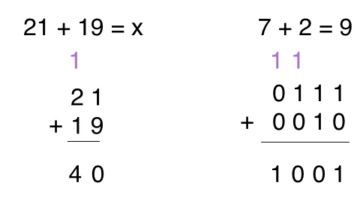
\includegraphics[scale=0.4]{binaryAddition.jpg}
% \end{frame}

% \begin{frame}{OK, but WHY does this work? (cont.)}
% \center
% Consider the following:

% \begin{tabular}{c@{\,}c@{\,}c@{\,}c@{\,}c@{\,}c@{\,}c@{\,}c@{\,}c@{\,}c} 
% {\color{red}1} & {\color{red}1} & {\color{red}1} & {\color{red}1} & & & & & \\
%  & 1 & 1 & 1 & 1 & 0 & 0 & 1 & 0 & (-14) \\
% $+$ & 0 & 0 & 0 & 1 & 1 & 0 & 0 & 1 & (25)\\ \hline
% {\color{red}1} & 0 & 0 & 0 & 0 & 1 & 0 & 1 & 1 & (11)\\ 
% \end{tabular}

% Since the overflow digit is lost, this can be said to work! 
% \end{frame}



\section[Linked Lists]{Linked Lists}
\begin{frame}{Singly Linked Lists}
A singly linked list is a graph where each node points to one other node, or no nodes, and no node is pointed to more than once.  
\begin{itemize}
\item This effectively creates a linear data structure.
\end{itemize}
\center
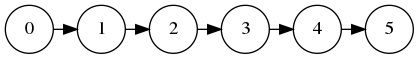
\includegraphics[scale=0.3]{SLL_simple.png}
\flushright
\begin{itemize}
\item This is similar in many respects to our old friend the array, but with some key differences.  
\item This is how languages such as Lisp and Haskell store lists, their primary native aggregate data type. 
\end{itemize}
\end{frame}

\begin{frame}[fragile=singleslide]{Linked Lists with Structures}
The nodes of the graph can be expressed as objects of a structure type in C.  All we need to do is take an existing structure and add the self-referential pointer \texttt{*next}...
\begin{lstlisting}[style=C]
struct SLLnode {
	char *name;
	char *email;
	int pinball;
	SLLnode *next;
};
\end{lstlisting} 
\begin{itemize}
\item The last element in the list points to \texttt{NULL}.
\item If we wish to refer to a singly linked list in \texttt{main()} or one of our functions, we need only a single node, from which we can access the rest.
\begin{lstlisting}[style=C]
struct SLLnode linkedList;
\end{lstlisting} 
\end{itemize}
\end{frame}

\begin{frame}{Linked Lists with Structures (cont.)}
If we apply our data structure to the singly linked list structure, we get the following:
\center
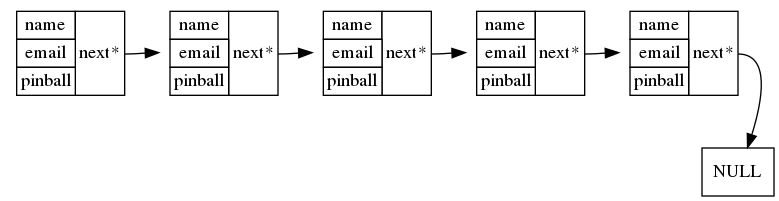
\includegraphics[scale=0.3]{SLL.png}
\flushleft
The more information that is contained in the structure, the more advantageous it is to organize it in this manner.  
\begin{itemize}
\item If you want to pass the first node by reference to a function, keep in mind that within the function you will have to dereference the argument to get to the first node's data. 
\end{itemize}
\end{frame}

\begin{frame}{Linked Lists vs Arrays}
So why go to all the bother?  Seems like a lot of work just to make something that functions roughly like an array.  
\begin{itemize}
\item Because the list is not stored in contiguous memory, it can be dynamically grown or shrunk \emph{without having to copy the whole array}.  
\item Because the next node is indicated with pointers, and those pointers may be modified, we can \emph{insert an element} without having to move any of the other elements in memory.  
\end{itemize}
However, there are some drawbacks.
\begin{itemize}
\item Because the nodes are not stored in contiguous memory, we can't perform pointer arithmetic to find a particular index.  
\begin{itemize}
\item Instead, we have to \emph{follow the node pointers.}
\item This means that finding the record at index \texttt{i} takes \texttt{i} operations, where an array can do it in 1.  
\end{itemize}
\end{itemize}
\end{frame}

\begin{frame}{Looking Back on Lists Past}
Singly linked lists are awesome, but you can only traverse them in one direction. 
\begin{itemize}
\item The \textbf{Doubly-Linked List} is a singly linked list, with the dded condition that each node has an edge that points to the node that points to it.  
\item No node may be pointed to more than twice.  
\end{itemize}
\center
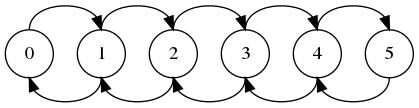
\includegraphics[scale=0.4]{DLL_simple.png}
\end{frame}

\begin{frame}[fragile=singleslide]{C Implementation}
With the addition of one more pointer, \texttt{*prev}, we have made a singly linked list node into a doubly linked list node.
\begin{lstlisting}[style=C]
struct DLLnode {
	char *name;
	char *email;
	int pinball;
	DLLnode *next;
	DLLnode *prev;
};
\end{lstlisting} 
\begin{itemize}
\item The first element's \texttt{prev} pointer will point to \texttt{NULL}
\item The last element's \texttt{next} pointer will also point to null.
\item While a doubly linked list increases the amount of bookkeeping, it makes the list traversable in either direction.  
\end{itemize}
\end{frame}

\begin{frame}{C Implementation (cont.)}
\center
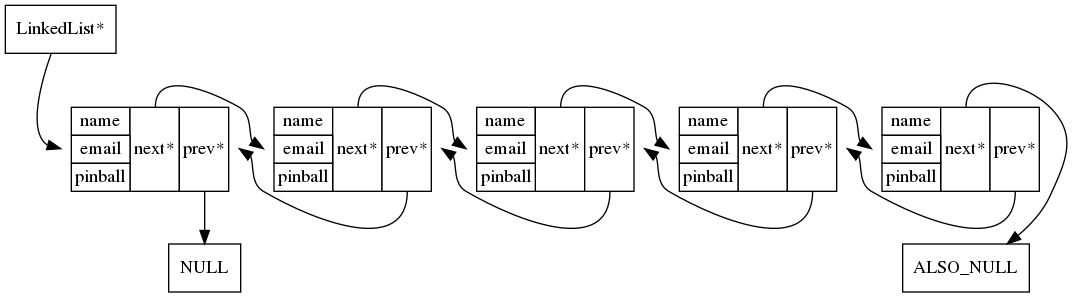
\includegraphics[scale=0.3]{DLL.png}
\end{frame}

\section[Trees]{Example: Binary Trees}
% \begin{frame}{Binary Trees!}
% \center
% 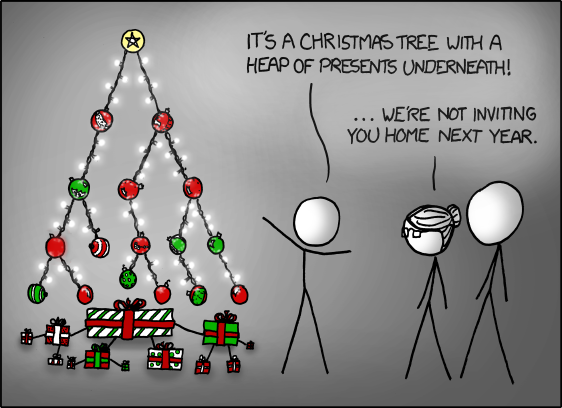
\includegraphics[scale=0.4]{tree.png}
% \end{frame}

\begin{frame}{Binary Trees!}
A \textbf{binary tree} is an acyclic, directed graph, where each node may connect to at most two others.  
\begin{columns}
\begin{column}{0.65\textwidth}
\begin{itemize}
\item Trees have a \textbf{root node}, here $R$
\begin{itemize}
\item The root of the tree is the node to which no other node points. 
\end{itemize}
\item For every vertex $v$, there is exactly one path to that vertex from the root node.  
\item Each node has exactly one \textbf{parent} (except for the root), and up to 2 \textbf{children}.  
\begin{itemize}
\item \emph{binary} tree nodes have $\leq 2$ children. 
\item \emph{n-ary} tree nodes have $\leq n$ children.
\end{itemize}
\end{itemize}
\end{column}
\begin{column}{0.35\textwidth}
\center
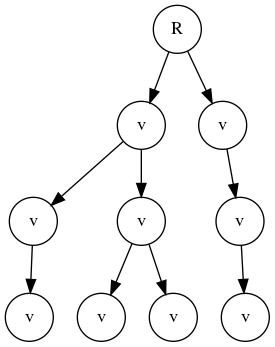
\includegraphics[scale=0.4]{tree1.png}
\end{column}
\end{columns}
\end{frame}

\begin{frame}{Binary Trees!}
\begin{itemize}
\item A \textbf{leaf node} is any node in the tree which does not point to any other nodes.
\item A \textbf{stem node} is any node in the tree which does point to other nodes.
\end{itemize}
\begin{columns}
\begin{column}{0.75\textwidth}
\begin{itemize}  
\item The \textbf{depth} of a tree is number of nodes in the longest branch.  (i.e., the distance from the root to the furthest leaf in nodes)
\item The nodes in a tree are organized into \textbf{levels}
\begin{itemize}
\item All the nodes of the same distance to the root node are at the same level.  
\end{itemize}
\item The \textbf{width} of a level is the number of nodes in that level.
\item A set of $n \geq 0$ disjoint trees is called a \textbf{forest}.
\end{itemize}
\end{column}
\begin{column}{0.25\textwidth}
\center
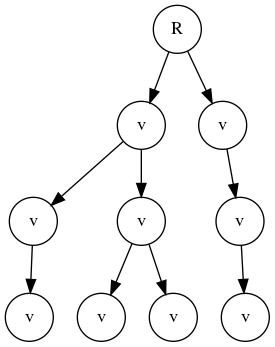
\includegraphics[scale=0.3]{tree1.png}
\end{column}
\end{columns}
\end{frame}


\begin{frame}[fragile=singleslide]{Implementation Considerations}
Whereas the singly linked list had only one ``next'' pointer, The binary tree has two.
\begin{itemize}
\item By convention, we call these \textbf{left} and \textbf{right}
\end{itemize}
\begin{lstlisting}[style=C]
struct  BinTree {
	int value;
	BinTree *left;
	BinTree *right;
};
\end{lstlisting} 
\begin{itemize}
\item One interesting property of trees is that they are a \emph{naturally inductive} data structure.
\begin{itemize}
\item i.e., both the nodes pointed to by \texttt{left} and \texttt{right} can be rightly considered roots of their own trees.  
\item Therefore, this is a natural application for \emph{recursive algorithms}.
\end{itemize}
\end{itemize}
\end{frame}

\begin{frame}[fragile=singleslide]{Tree Summing Algorithm}
Let's design an algorithm to recursively sum all the values in a tree!

The sum of a tree is the sum of the left tree, the right tree and the value of the root node.
\begin{enumerate}
\item If the left tree doesn't exist (i.e., is a null pointer), it's sum is zero.
\item If the left tree exists, we recursively call the summing function on the left tree, considering the node pointed to by the left pointer to be the new root node in this recursive call.  We hold onto the return value for later.
\item We repeat steps 2 and 3 with the right tree.
\item We add the results of step 2 and 3 to the value of the root node, and return this value. 
\end{enumerate}
\end{frame}

\begin{frame}{Example: Summing the Values in a Tree}
\begin{columns}
\begin{column}{0.33\textwidth}
\center
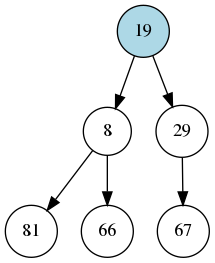
\includegraphics[scale=0.3]{summing_tree_1.png}
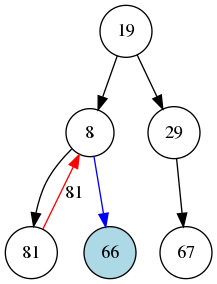
\includegraphics[scale=0.3]{summing_tree_4.png}
\end{column}
\begin{column}{0.33\textwidth}
\center
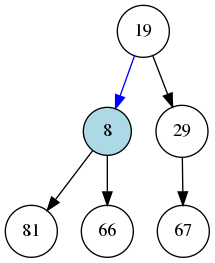
\includegraphics[scale=0.3]{summing_tree_2.png}
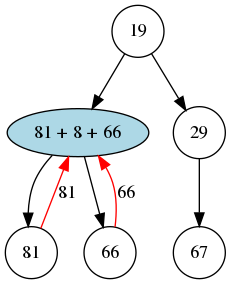
\includegraphics[scale=0.3]{summing_tree_5.png}
\end{column}
\begin{column}{0.33\textwidth}
\center
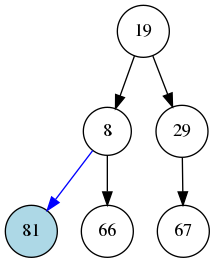
\includegraphics[scale=0.3]{summing_tree_3.png}
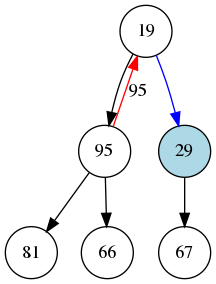
\includegraphics[scale=0.3]{summing_tree_6.png}
\end{column}
\end{columns}
\end{frame}

\begin{frame}{Example: Summing the Values in a Tree (cont.)}
\center
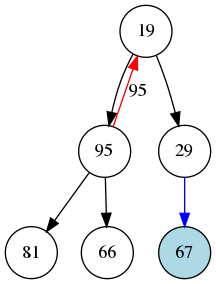
\includegraphics[scale=0.28]{summing_tree_7.png} \hspace{1em}
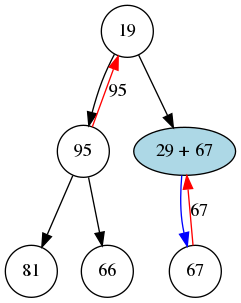
\includegraphics[scale=0.28]{summing_tree_8.png} \hspace{1em}
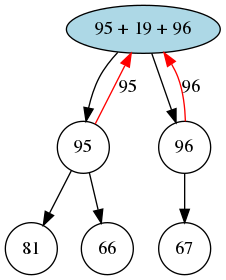
\includegraphics[scale=0.28]{summing_tree_9.png} \hspace{1em}
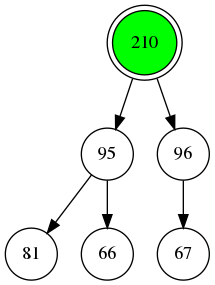
\includegraphics[scale=0.28]{summing_tree_10.png}

This example overwrites node values with the results of summation.  This is mostly for demonstration purposes, a real algorithm wouldn't overwrite node contents like this! 
\end{frame}

\begin{frame}{Depth vs Breadth First Search}
Searching a tree can go very differently depending on how you approach it.
\begin{itemize}
\item \textbf{Depth-First Search} (DFS)
\begin{itemize}
\item Selects a branch and follows it until a leaf node is found.
\item If a leaf is reached without the searched-for item being found, DFS backtracks to the last node it made a branch decision on (with untried branches) and tries another branch.
\item Suitable for exploring decision branches in game AI
\end{itemize}
\item \textbf{Breadth-First Search} (BFS)
\begin{itemize}
\item Searches all of the nodes in one level of the tree before moving on to the next.  
\item Requires more traversal / bookkeeping than DFS.
\item Finds minimum branch depth much faster than DFS.  
\end{itemize}
\end{itemize}
DFS vs BFS is a popular topic among people who think computer algorithms have applications to human behaviour.  
\end{frame}

\begin{frame}{Binary Search Trees!}
Both DFS and BFS assume nothing about the structure of the data contained in the tree (aside from the fact it is a tree).
If we give trees certain mathematical properties, we can write algorithms that vastly improve general-case runtimes! 
\vspace{1em}
\begin{columns}
\begin{column}{0.75\textwidth}
The \textbf{Binary Search Tree Property} is as follows:
\begin{itemize}
\item If a node has a left child node, the value of that node is less than or equal to the value of the parent node.
\item If a node has a right child node, the value of that node is greater than the parent node.  
\end{itemize}
\end{column}
\begin{column}{0.25\textwidth}
\center
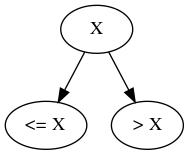
\includegraphics[scale=0.3]{BST_simple.png}
\end{column}
\end{columns}
\vspace{0.5em}
Depending on who writes the definition, duplicate elements are sometimes disallowed.
\end{frame}

\begin{frame}{Binary Search Trees: Pros and Cons}
Pros:
\begin{itemize}
\item Best case scenario runtime for search, insertion and deletion operations is $O(d)$, Where $d$ is the depth of the tree.
\begin{itemize}
\item In the best case scenario, the depth of the tree is $log_2(n)$, where $n$ is the number of nodes.  
\end{itemize}
\end{itemize}
Cons:
\begin{itemize}
\item The worst case scenario for $d$ is $n$
\begin{itemize}
\item This is a tree with only one branch, (basically a linked list).  
\end{itemize}
\item The search tree property is maintained, which requires some extra book-keeping.  
\end{itemize}
To address the drawbacks of unbalanced trees, BSTs in practice often use \emph{balancing algorithms}, such as \textbf{Red Black Trees} or \textbf{Adelson-Velsky and Landis (AVL) Trees}.
\end{frame}

\section[Graphs]{Graph Theory}
\begin{frame}{A Brief Introduction to Graph Theory}
In order to solve problems, we need mathematical models in which to express those problems.  A very useful mathematical model used in algorithm design is the \textbf{graph}.
\begin{itemize}
\item A graph is a way of modelling the relationships between objects.
\item A graph is defined (mathematically) as the ordered pair: 
$$ G = (V, E) $$
\item Where $V$ is the set of  \textbf{nodes} or \textbf{vertices}, and
\item Is the set of edges, conforming to : 
$$E \subseteq \{\{x,y\} | x,y \in V \wedge x \neq y\} $$
\item The above means that an edge is defined as a pair of vertices, where the two vertices may not be the same. 
\end{itemize}
\end{frame}

\begin{frame}{Here's an Example...}
\center 
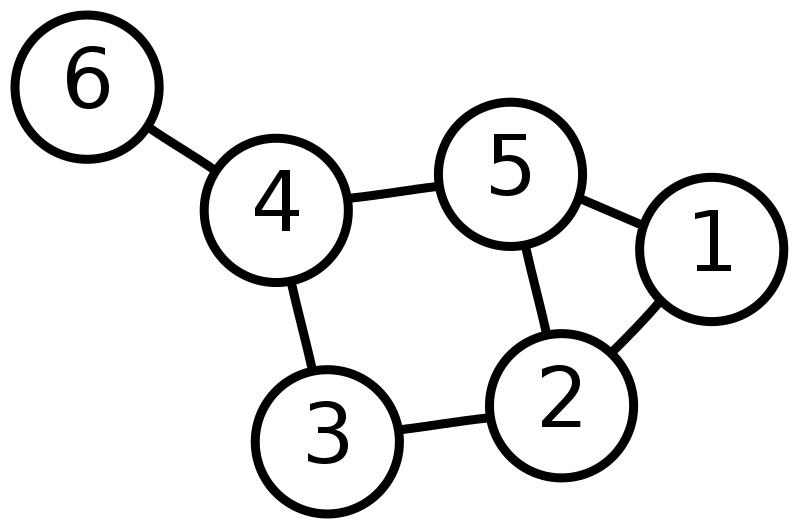
\includegraphics[scale=0.2]{graph.png}
\flushleft
In the above...
\begin{itemize}
\item $V = \{1,2,3,4,5,6\}$
\item $E = \{\{6,4\},\{4,5\},\{4,3\},\{5,1\},\{5,2\},\{3,2\},\{1,2\}\}$
\end{itemize}
\end{frame}

\begin{frame}{Directed Graphs}
The previous two slide present graphs in their most general form.  If we apply properties to graphs, we get some interesting structures.  
\begin{itemize}
\item Directed Graphs:
\begin{itemize}
\item If ordering of the numbers in an edge pair matters, the graph is \textbf{directed}.  
\item Simply put, the graph has \emph{arrows} instead of \emph{straight lines}.  
\end{itemize}
\item Cyclic vs Acyclic Graphs:
\begin{itemize}
\item A cyclic graph contains \textbf{cycles}.
\item If it is possible to return to any node by following the edges of a directed graph, then the graph is \textbf{cyclic}.
\item Otherwise it is \textbf{acyclic} (ay-sick-lick).
\end{itemize}
\end{itemize}
\end{frame}

\begin{frame}{Directed Graphs}
\begin{columns}
\begin{column}{0.5\textwidth}
\center
\textbf{Directed, Cyclic Graph}
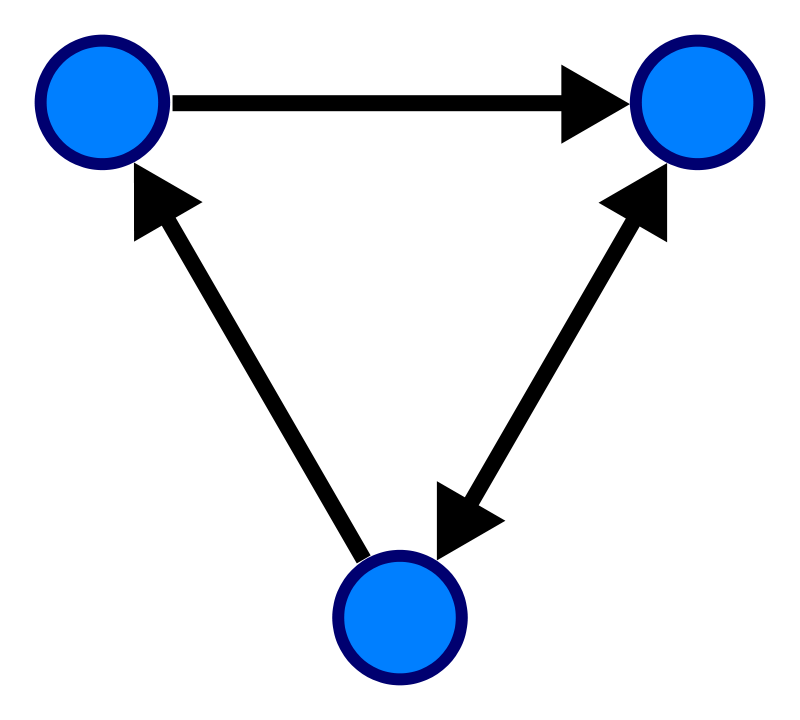
\includegraphics[scale=0.1]{directed.png}
\end{column}
\begin{column}{0.5\textwidth}
\center
\textbf{Directed, Acyclic Graph}
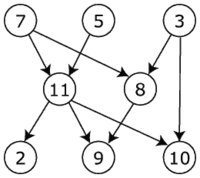
\includegraphics[scale=0.4]{directedAcyclic.png}
\end{column}
\end{columns}
Graphs have lots more properties than this, but this will do for now.
\begin{itemize}
\item In the context of C programming, we can make \emph{nodes} with structures
\item If our structure contains a pointer to another structure of the same type, this can be considered an \emph{edge}.  
\end{itemize}
\end{frame}

\section[Acknowledge]{Acknowledge}
\begin{frame}{Acknowledge}
\center
\vspace{8em}
The contents of these slides were liberally borrowed (with permission) from slides from the Summer 2021 offering of 1XC3 (by Dr. Nicholas Moore).  
\end{frame}

\end{document}